%\chapwithtoc{Appendix}

\begin{appendices}

\chapter{Invariant differential operators for $(2,3,5)$-distributions}


\section{The (2,3,5) distribution}

The famous Cartan $(2,3,5)$ distribution corresponds to the pair $(G_2, P_1)$.

\subsection{Singular vectors --- polynomials}

Dimensions of graded components of our nilradical are $2, 1, 2$ and we introduce variables $x_1, x_2, y, z_1, z_2$ that reflect this grading. We take a finite-dimensional representation of the semisimple part of the Levi subgroup of $P_1$ which is in this case determined by a nonnegative number $a$ and extend it to the whole Levi subgroup by decreeing the center to act by zero. In the embedding into the Lie algebra of $G_2$ this corresponds to $\sigma = -\frac{3}{2} \omega_1 + a \omega_2$ since the central element is $h_c = 2h_1 + 3h_2$.

Using the formula (??) of \cite{ks_2015} we calculate the action of the basis vectors on the polynomial realization of our Verma module $M(\sigma_{\lambda-\rho})$ induced from representation $\sigma$ twisted by scalar representation of weight $\lambda + \rho$.

Action of the Levi subalgebra:
\begin{align}
    \actpol(e) &= x_1 \pd{x_2} - z_1 \pd{z_2} + \sigma(e) \\
    \actpol(f) &= x_2 \pd{x_1} - z_2 \pd{z_1} + \sigma(f)\\
    \actpol(h) &= x_1 \pd{x_1} - x_2 \pd{x_2} + z_1 \pd{z_1} - z_2 \pd{z_2} + \sigma(h) \\
    \actpol(h_c) &= (2\lambda -5) - (2 \euler_y + \euler_x + 3 \euler_z)
\end{align}

Since the equations for singular vectors are invariant with respect to the semisimple part of the Levi subalgebra, our strategy is to decompose the space of polynomials with respect to $\lie{l}$ and solve the equations on the isotypical components.

According to Riesz-Fischer \cite{RF_1920} we can write the polynomial algebra $\mathbb{C}[x_1,x_2,y,z_1,z_2]$ as $\mathbb{C}[y,q] \otimes \mathcal{H}$, where $y$ and \[q = x_1z_2 + x_2 z_1\] are the only polynomials invariant with respect to the action of $\lie{l}$. The space $\mathcal{H}$ is the intersection of kernels of differential operators obtained as the Fourier images of $y$ and $q$. Namely $\pd{y}$ and
\[\lap = \pd{x_1}\pd{z_2} + \pd{x_2}\pd{z_1}.\]
Later on we will work with a particular invariant polynomial $(y^2 - 4q)^k$ for which we have identity
\[
\lap (y^2 - 4q)^k = -8k(y^2 - 4q)^{k-2}(y - 2(k+1)q).
\]
Moreover, we have a finer decomposition of $\mathcal{H}$ with respect to our $\mathfrak{sl}_2$ action:
\begin{equation}
    \mathcal{H} = \bigoplus_{a,b} \mathcal{H}_{a,b},
\end{equation}
where $\mathcal{H}_{a,b}$ is the space of harmonic polynomials which are $a$-homogeneous in $x_1, x_2$ and $b$-homogeneous in $z_1, z_2$. It is an irreducible $\mathfrak{sl}_2$ module with highest weight $a+b$ and highest weight vector $x_1^a z_1^b$. %TODO zkontrolovat

%As follows from the action of the central element $c$ of our Levi subalgebra, the singular vectors must have constant weighted degree.
\begin{align}
    \wdeg y = 2 & \quad  \wdeg q = 4 \\
    \wdeg x_i = 1 & \quad  \wdeg z_i = 3
\end{align}
%Thus polynomial of the form $y^kq^lx_i^az_j^b$ has weighted degree $2k + 4l + a + 3b$ and normal degree $k+2l+a+b$.

Action of the first graded component:
\begin{align}
    \actpol(e_1) &= -2 x_2 \pd{y} - y \pd{z_1} \\
             & \quad + \frac{3}{2} (z_1 \pd{x_1} - z_2 \pd{x_2}) \pd{z_1} + \left(\euler_x + \frac{1}{2}\euler_y + \frac{5}{2} - \lambda\right)\pd{x_1} \\
             & \quad + \frac{3}{2} \pd{x_1}\sigma(h) + 3 \pd{x_2} \sigma(f) \\
             & \quad - \frac{1}{4} (z_1 \pd{x_1} - z_2\pd{x_2})\pd{x_1}\pd{y}\\
    \actpol(e_2) &= 2 x_1 \pd{y} + y \pd{z_2} \\
             & \quad - \frac{3}{2} (z_1 \pd{x_1} - z_2 \pd{x_2}) \pd{z_2} + \left(\euler_x + \frac{1}{2}\euler_y + \frac{5}{2} - \lambda\right)\pd{x_2} \\
             & \quad - \frac{3}{2} \pd{x_2} \sigma(h) + 3 \pd{x_1} \sigma(e) \\
             & \quad - \frac{1}{4} (z_1 \pd{x_1} - z_2 \pd{x_2})\pd{x_2}\pd{y}
\end{align}

We define three auxiliary operators
\begin{align}
    P_+ & = x_1 \pd{z_1} - x_2 \pd{z_2} \\
    P_- & = z_1 \pd{x_1} - z_2 \pd{x_2} \\
    P_0 & = [P_+, P_-] = \euler_x - \euler_z
\end{align}
which satisfy $\lie{sl}_2$ relations: $[P_0, P_+] = 2P_+$, $[P_0, P_-] = 2P_-$ and are invariant with respect to the semisimple Levi %TODO

We can use the following commutation relations:
\begin{align}
P_- x_1 & = x_1 P_- + z_1 & \quad P_- \pd{z_1} = \pd{z_1} P_- - \pd{x_1} \\
P_- x_2 & = x_2 P_- - z_2 & \quad P_- \pd{z_2} = \pd{z_2} P_- + \pd{x_2}
\end{align}

Another useful operators (commutant?)
\begin{align}
Q_- &= \pd{x_1}^2 \sigma(e) - \pd{x_2}^2 \sigma(f) - \pd{x_1}\pd{x_2} \sigma(h) \\
Q_+ &= x_2^2 \sigma(e) - x_1^2 \sigma(f) + x_1 x_2 \sigma(h) \\
C &= 2(\cas + x_2\pd{x_1} \sigma(e) + x_1\pd{x_2}\sigma(f) + \frac{1}{2}(x_1\pd{x_1} - x_2\pd{x_2})\sigma(h))
\end{align}
where
\begin{equation}
\cas = \sigma(e)\sigma(f) + \sigma(f)\sigma(e) + \frac{1}{2} \sigma(h)^2.
\end{equation}

The following commutation relations hold
\begin{gather}
    \begin{align}
        [\euler_x, Q_+] &= 2Q_+    &  [Q_+, C] &= \euler_x Q_+  \\
        [\euler_x, Q_-] &= -2Q_-   &  [Q_-, C] &= -Q_- \euler_x
    \end{align}\\
    [Q_+, Q_-] = (\euler_x + 1) C
\end{gather}

\begin{align}
[Q_+, P_+] = 0 \quad [Q_+, q] = 0 \quad [Q_-, P_-] = 0 \quad [Q_-, \lap] = 0
\end{align}

\begin{align}
    [Q_-, q] &= - (z_1\pd{x_1}+z_2\pd{x_2})\sigma_h + 2z_2\pd{x_1}\sigma(e) - 2z_1\pd{x_2}\sigma(f)  \\
    [Q_+, \lap] &= -(x_1\pd{z_1} + x_2\pd{z_2}) \sigma(h) + 2x_1\pd{z_2}\sigma(f) - 2x_2\pd{z_1}\sigma(e)
\end{align}

\begin{align}
[Q_+, P_-] &= (x_1z_2 - x_2z_1)\sigma(h) + 2x_2z_2\sigma(e) + 2x_1z_1\sigma(f)\\
[Q_+, P_-] &= q\sigma(h) + 2\left(x_2z_2\sigma(e) + x_1z_1\sigma(f) -x_2z_1\sigma(h) \right)\\
[Q_-, P_+] &= (\pd{x_1}\pd{z_2} - \pd{x_2}\pd{z_1})\sigma(h) + 2\pd{x_1}\pd{z_1}\sigma(e) + 2\pd{x_2}\pd{z_2}\sigma(f) \\
[Q_-, P_+] &= \lap\sigma(h) + 2\left(\pd{x_1}\pd{z_1}\sigma(e) + \pd{x_2}\pd{z_2}\sigma(f) - \pd{x_2}\pd{z_1} \sigma(h)\right)\\
[C, P_+] &= (x_1\pd{z_1} + x_2 \pd{z_2})\sigma(h) - 2x_1\pd{z_2}\sigma(f) + 2x_2 \pd{z_1} \sigma(e) \\
[P_-, C] &= (z_1\pd{x_1} + z_2 \pd{x_2})\sigma(h) + 2 z_1\pd{x_2}\sigma(f) - 2z_2 \pd{x_1} \sigma(e)
\end{align}

\begin{align}
[Q_-, \actpol(e_1)] & = \pd{x_1}(- Q_- + 2\pd{y}\sigma(h) ) + 4\pd{y}\pd{x_2}\sigma(f) \\
[Q_-, \actpol(e_2)] & = \pd{x_2}( - Q_- -2\pd{y}\sigma(h)) + 4\pd{y}\pd{x_1}\sigma(e)
\end{align}

\begin{align}
 [Q_-, [Q_-, q]] & = 2P_-Q_-\\
 [q, [q, Q_-]] & = 2Q_+^z
\end{align}

\[
 [\lap, [Q_-^x, q]] = 2Q_-^x
\]

\begin{align}
Q_-^z &= \pd{z_1}^2 \sigma(e) - \pd{z_2}^2 \sigma(f) + \pd{z_1}\pd{z_2} \sigma(h) \\
Q_+^z &= z_2^2 \sigma(e) - z_1^2 \sigma(f) - z_1 z_2 \sigma(h)
\end{align}


\begin{align}
[Q_-^x, Q_-^z] & = \lap[(\pd{x_1}\pd{z_2} - \pd{x_2}\pd{z_1}) \sigma(h) + 2\pd{x_2}\pd{z_2}\sigma(f) + 2\pd{x_1}\pd{z_1}\sigma(e)] \\
[Q_+^x, Q_+^z] & = q[(x_1 z_2 - x_2 z_1) \sigma(h) + 2x_1 z_1 \sigma(f) + 2x_2 z_2 \sigma(e)] \\
[Q_+^z, Q_-^x] & = P_-[(z_1\pd{x_1} + z_2 \pd{x_2})\sigma(h) + 2 z_1\pd{x_2}\sigma(f) - 2z_2 \pd{x_1} \sigma(e)] \\
[Q_+^x, Q_-^z] & = P_+[(x_1\pd{z_1} + x_2 \pd{z_2})\sigma(h) - 2x_1\pd{z_2}\sigma(f) + 2x_2 \pd{z_1} \sigma(e))]
\end{align}

\begin{align}
[Q_-^x, Q_-^z] & = \lap [Q_-^x, P_+] \\
[Q_+^x, Q_+^z] & = q [Q_+^x, P_-] \\
[Q_+^z, Q_-^x] & = -P_-[C, P_-] \\
[Q_+^x, Q_-^z] & = P_+[C, P_+]
\end{align}

Now we can rewrite the action as follows:
\begin{align}
    \actpol(e_1) &= -2 x_2 \pd{y} - y \pd{z_1} \\
             & \quad + \frac{3}{2} P_- \pd{z_1} + ( \euler_x + \frac{1}{2}\euler_y + \frac{5}{2} - \lambda)\pd{x_1} \\
             & \quad + \frac{3}{2} \pd{x_1}\sigma(h) + 3 \pd{x_2} \sigma(f) \\
             & \quad - \frac{1}{4} P_- \pd{x_1}\pd{y}\\
    \actpol(e_2) &= 2 x_1 \pd{y} + y \pd{z_2} \\
             & \quad - \frac{3}{2} P_- \pd{z_2} + ( \euler_x + \frac{1}{2}\euler_y + \frac{5}{2} - \lambda)\pd{x_2} \\
             & \quad - \frac{3}{2} \pd{x_2} \sigma(h) + 3 \pd{x_1} \sigma(e) \\
             & \quad - \frac{1}{4} P_- \pd{x_2}\pd{y}
\end{align}

Since the second degree part $\lie{g}_2$ is one-dimensional, we get a $\lie{sl}_2$-invariant differential operator.
\begin{align}
[\actpol(e_1), \actpol(e_2)] & = 2 P_+ - \frac{3}{2}P_-\pd{y}^2 + 2y\lap \\
& \quad + (5\euler_x + 2\euler_y + 3\euler_z + 10 - 4\lambda)\pd{y} \\
& \quad + (z_2\pd{z_2} - z_1\pd{z_1})\pd{x_1}\pd{x_2} + z_2\pd{z_1}\pd{x_2}^2 - z_1\pd{z_2}\pd{x_1}^2 \\
& \quad + 3\left(\pd{x_1}\pd{x_2}\sigma(h) + \pd{x_2}^2 \sigma(f) - \pd{x_1}^2 \sigma(e) \right) \\
& \quad + \left[\frac{3}{2} \pd{x_1}\sigma(h) + 3 \pd{x_2} \sigma(f), - \frac{3}{2} \pd{x_2} \sigma(h) + 3 \pd{x_1} \sigma(e) \right].
\end{align}
The last term is a Lie bracket which can be rewritten as
\begin{equation}
9\left(\pd{x_1}^2\sigma(e) - \pd{x_2}^2\sigma(f) - \pd{x_1}\pd{x_2}  \sigma(h) \right).
\end{equation}
Combining the vectorial terms together we obtain after some further manipulation
\begin{align}
[\actpol(e_1), \actpol(e_2)] & = 2 P_+ - \frac{3}{2}P_-\pd{y}^2 + 2y\lap \\
& \quad + (5\euler_x + 2\euler_y + 3\euler_z + 10 - 4\lambda)\pd{y} \\
& \quad - P_- \lap\\
& \quad - 6\left(\pd{x_1}\pd{x_2}\sigma(h) + \pd{x_2}^2 \sigma(f) - \pd{x_1}^2 \sigma(e) \right)
\end{align}

Now we look at some interesting combinations.
\begin{align}
x_1 \actpol(e_1) + x_2 \actpol(e_2) &= -y P_+ \label{eq:comb1}\\
        & \quad \frac{3}{2}(P_-P_+ - \euler_z)  + (\euler_x + \frac{1}{2}\euler_y + \frac{3}{2} - \lambda)\euler_x \label{eq:comb1a}\\
        & \quad \frac{3}{2}(x_1\pd{x_1} - x_2\pd{x_2}) \sigma(h) \\
        & \quad + 3x_1\pd{x_2}\sigma(f) + 3x_2\pd{x_1}\sigma(e) \\
        & \quad - \frac{1}{4}P_- (\euler_x - 1) \pd{y}
\end{align}


\begin{align}
z_1 \actpol(e_1) - z_2 \actpol(e_2) &= -2q\pd{y} - y \euler_z \label{eq:comb2}\\
        & \quad \left( \euler_x + \frac{1}{2}\euler_y  + \frac{3}{2}\euler_z + 1 - \lambda \right) P_-\\
        & - \frac{3}{2} [Q_-, q] \\
        & \quad + \frac{3}{2}(z_1\pd{x_1} + z_2\pd{x_2})\sigma(h) \\
        & \quad + 3 z_1 \pd{x_2} \sigma(f) - 3 z_2 \pd{x_1} \sigma(e) \\
        & \quad -\frac{1}{4}P_-^2 \pd{y}
\end{align}

\begin{align}
\pd{z_2} \actpol(e_1) + \pd{z_1} \actpol(e_2) &= 2 P_+\pd{y} \\
        & \quad \dots
2\end{align}

\begin{align}
\pd{x_2} \actpol(e_1) - \pd{x_1} \actpol(e_2) &= -2 (\euler_x + 2)\pd{y} - y \lap\\
        & \quad + \frac{3}{2} \lap P_- \\
        & \quad + 3 ( \pd{x_1} \pd{x_2} \sigma(h) + \pd{x_2}^2 \sigma(f) - \pd{x_1}^2 \sigma(e))
\end{align}

We see that $[\actpol(e_1), \actpol(e_2)] + 2(\pd{x_2} \actpol(e_1) - \pd{x_1} \actpol(e_2))$ is
\begin{equation} \label{eq:vector-free}
2(P_+ + \lap P_-) - \frac{3}{2}P_- \pd{y}^2 + \pd{y}(\euler_x + 2\euler_y + 3\euler_z - 4\lambda).
\end{equation}

\begin{align}
x_1 \actpol(e_1) + x_2 \actpol(e_2) &= -y P_+ \\
        & \quad \frac{3}{2}(P_-P_+ - \euler_z)  + (\euler_x + \frac{1}{2}\euler_y + \frac{3}{2} - \lambda)\euler_x \label{eq:comb1a}\\
        & \quad \frac{3}{2} C - Cas_\mathbb{V} \\
        & \quad - \frac{1}{4}P_- (\euler_x - 1) \pd{y}
\end{align}

\begin{align}
-z_1 \actpol(e_1) + z_2 \actpol(e_2) &= 2q\pd{y} + y \euler_z \\
        & \quad -P_-\left( \euler_x + \frac{1}{2}\euler_y  + \frac{3}{2}\euler_z + \frac{3}{2} - \lambda \right)\\
        & \quad +\frac{3}{2}[Q_-, q] \\
        & \quad +\frac{1}{4}P_-^2 \pd{y}
\end{align}

\bigskip
\hrule
\bigskip

Consider the homogeneous part $\vsingtop$ of a singular vector with the highest (nonweighted) degree. Since \eqref{eq:comb1} is the only part of the operator $x_1\actpol(e_1) + x_2\actpol(e_2)$ that raises degree, the polynomial $\vsingtop$ must be in the kernel of $P_+$. In other words, the harmonic part of $\vsingtop$ is contained in $\mathcal{H}_{a,0}$ and in particular it means that the harmonic part is free of $z$ variables. Now we can use the action of $z_1\actpol(e_1) - z_2\actpol(e_2)$ on $\vsingtop$ to derive the equation for ``the invariant part'' of the top-degree component of singular vectors:
\[
(2q\pd{y} + y\euler_z) p(q,y) = 0.
\]%TODO
We CLAIM that all solutions are of the form $(y^2 - 4q)^k$ for some $k\in\mathbb{N}$. To summarize, the top-degree part of any singular vector lies in the space $\mathbb{C}[y^2 - 4q]_k \otimes \mathcal{H}_{a,0} \otimes \mathbb{V}$. The whole singular vector must be homogeneous with respect to the weighted degree, which in this case is $4k + a$. A subleading term of degree $2k + a - l$ consists of monomials of the form $y^{k_1}q^{k_2} p \otimes v$ where $p$ is an element of $\mathcal{H}_{b,c}$. Such a monomial has a weighted degree of $2k_1 + 4k_2 + b + 3c$. Hence we obtain the following system of equations
\begin{align}
 2k_1 + 4k_2 + b + 3c & = 4k + a \\
  k_1 + 2k_2 + b +  c & = 2k + a - l
\end{align}
whose difference is
\[
k_1 + 2k_2 + 2c = 2k + l.
\]
% The only way to cancel out the result of \eqref{eq:comb1a} on $\vsingtop$ is to match it with the action of \eqref{eq:comb1} on the subleading term. It follows that the subleading term must be contained in $\mathcal{H}_{a-1,1}$ and have degree in $y$ one less.

\bigskip
\hrule
\pagebreak
\bigskip

Leading term
\[
    (y^2-4q)^k \otimes H_{a,0} \otimes V
\]

Subleading term of degree one less is contained in $(\mathbb{C}[y^2, q]_m \oplus y\mathbb{C}[y^2, q]_m)\otimes H_{c,d} \otimes V$.

The weighted homogeneity of the first part must match the weighted homogeneity of the leading term.
\[
4m + c + 3d = 4k + a.
\]
If we substract the equation for degree
\[
2m + c + d = 2k + a - 1,
\]
we get $2m + 2d = 2k + 1$ which is a contradiction.

Analogously for the second term
\begin{gather*}
4m + c + 3d + 2 = 4k + a \\
2m + c + d + 1= 2k + a - 1.
\end{gather*}
Substracting gives us $ m + d = k $. This allows us to write the subleading term as
\[
y\mathbb{C}[y^2, q]_{k-d}\otimes H_{a+d-2, d} \otimes V
\]
where $d = \max(0, 2-a), \ldots, k$.

Applying the equation \eqref{eq:vector-free} and looking at the subleading and leading term we get
\begin{align}
\mathrm{LT} &\longrightarrow 2k(4k - 4\lambda + a)y(y^2-4q)^{k-1}\otimes H_{a,0} \otimes V \\
\mathrm{SLT} &\longrightarrow 2y\mathbb{C}[y^2, q]_{k-d}H_{a+d-1, d-1} \otimes V
\end{align}
We immediately see that the subleading term can have only $d \in \{0, 1\}$. This gives the following three cases:
\begin{enumerate}
\item $a=0$ no subleading term $\Rightarrow$ $k=0 \vee \lambda = k$ The case $k=0$ gives only the generating vector of our Verma module and for the case $k=\lambda$ we apply \eqref{eq:comb2}. The only nontrivial question is whether $[Q_-, q]$ gives zero, but action of this commutator simplifies in our ansatz to $ky(y^2-4q)^{k-1}Q_+^z V$ and since $Q_+^z$ is $\mathfrak{sl}_2$-invariant the result is zero if and only if  our inducing representation $V$ is trivial. It is then straightforward to verify that any power of $y^2-4q$ really is a singular vector for a scalar parabolic Verma module.
\item $a=1$ $\Rightarrow$ $d=1$ and the subleading term is in the space
\[
    -(4k+1-4\lambda)ky(y^2-4q)^{k-1}\otimes P_- H_{1,0}
\]
Result of application of \eqref{eq:comb2} on the subleading term
\[
    (2q\pd{y} + y\euler_z) \left[ (4k+1-4\lambda)ky(y^2-4q)^{k-1}\otimes P_- H_{1,0} \otimes V \right]
\]
must cancel out with the corresponding action on the leading term
\[
\left((\euler_x + \frac{1}{2}\euler_y + \frac{3}{2}\euler_z + 1 - \lambda)P_- \oplus (-\frac{3}{2}[Q_-,q] \right) (y^2-4q)^k\otimes H_{1,0}\otimes V
\]
\item $a \geq 2$ $\Rightarrow$ $d=1 \vee d=0$ where we don't obtain any condition for the $d=0$ part and the $d=1$ is similarly to the previous case given by
\[
    -\frac{(4k+a-4\lambda)ky(y^2-4q)^{k-1}}{a}\otimes P_- H_{a,0}
\]
and the subleading term can have one more nontrivial part from
\[
    y\mathbb{C}[y^2,q]_k\otimes H_{a-2,0}
\]
\end{enumerate}

\[
    [\lap, [Q_-,q]] = 2[\pd{x_1}^2\sigma(e) - \pd{x_2}^2\sigma(f) - \pd{x_1}\pd{x_2}\sigma(h)]
\]

\bigskip
\hrule
\bigskip

Action of the Levi subalgebra on scalar Verma modules:
\begin{align}
    \actpol(e) &= x_1 \pd{x_2} - z_1 \pd{z_2} \\
    \actpol(f) &= x_2 \pd{x_1} - z_2 \pd{z_1} \\
    \actpol(h) &= x_1 \pd{x_1} - x_2 \pd{x_2} + z_1 \pd{z_1} - z_2 \pd{z_2} \\
    \actpol(c) &= (2\lambda -5) - (2 \euler_y + \euler_x + 3 \euler_z)
\end{align}

\chapter{Source code}

The Bruhat graphs in this work were produced with the help of the following code written for the mathematical software called sage \cite{sage}. Most of the code was submitted in a form of patch with respect to the version 5.12.

\begin{minted}[fontsize=\footnotesize]{python}
def minimal_representatives(self, index_set = None, side="right"):
  """
  Returns the set of minimal coset representatives of ``self``
  by a parabolic subgroup. 

  INPUT:

  - ``index_set`` - a subset (or iterable) of the nodes of the dynkin diagram,
		    empty by default
  - ``side`` - 'left' or 'right' (default)

  See documentation of ``self.bruhat_poset`` for more details.

  The output is equivalent to ``set(w.coset_representative(index_set,side))``
      
  but this routine is much faster. 
  For explanation of the algorithm see e.g. Cap, Slovak: Parabolic geometries, p. 332

  EXAMPLES::
      
      sage: G = WeylGroup(CartanType("A4"),prefix="s")
      sage: index_set = [1,3,4]
      sage: side = "left"
      sage: a = set(w for w in G.minimal_representatives(index_set,side))
      sage: b = set(w.coset_representative(index_set,side) for w in G)
      sage: print a.difference(b)
      set([])
  """
  from sage.combinat.root_system.root_system import RootSystem
  from copy import copy
  
  if side != 'right' and side != 'left':
      raise ValueError, "%s is neither 'right' nor 'left'"%(side)
  
  weight_space = RootSystem(self.cartan_type()).weight_space()
  if index_set == None:
      crossed_nodes = set(self.index_set())
  else:
      crossed_nodes = set(self.index_set()).difference(index_set)
  # the characteristic vector
  rhop = sum([weight_space.fundamental_weight(i) for i in  crossed_nodes]) 
  '''
  The varibale "todo" serves for traversing the orbit of rhop, 
  while the directory "known" serves as a memory to keep the visited elements.
  Its keys are elements in the orbit of rhop while known[vec] are paths of 
  simple reflections from rhop to vec.
  '''
  todo = [rhop]
  known = dict()
  known[rhop] = []
  if rhop == 0:
      return set( [self.one()] )
  else:
      while len(todo) > 0:
	  vec = todo.pop()
	  nonzero_coeffs = [i for i in self.index_set() if vec.coefficient(i) > 0]
	  for i in nonzero_coeffs:
	      new_vec = vec.simple_reflection(i)
	      new_reflections = copy(known[vec])
	      new_reflections.append(i)
	      todo.append(new_vec)
	      known[new_vec] = new_reflections
      if side =='left':
	  return set(self.from_reduced_word(w) for w in known.values())
      else:
	  # here we could just take the inverses of w 
	  # but reversing the list of simple reflections is slightly more efficient
	  return set(self.from_reduced_word(w[::-1]) for w in known.values()) 
	  
def parabolic_bruhat_graph(self, index_set = None, side="right"):
  """
  Returns the Hasse graph of the poset ``self.bruhat_poset(index_set,side)``
  with edges labeled by the cover relation.
  """
  elements = minimal_representatives(index_set, side)
  covers =[(x,y)  for y in elements for x in y.bruhat_lower_covers() if x in elements]
  res = DiGraph()
  for u,v in covers:
      res.add_edge(u,v,v.inverse()*u)
  return res         
  
def bruhat_poset(self, index_set = None, side="right", facade = False):
  """
  Returns the Bruhat poset of minimal coset representatives of ``self`` by a parabolic 
  subgroup.
  
  INPUT:
  
  - ``index_set`` - a subset (or iterable) of the nodes of the dynkin diagram, empty by default
  - ``side`` - 'left' or 'right' (default)
  
  Let W_S be the subgroup of W (``self`` ) that is generated by the simple reflections 
  corresponding to the set S (``index_set``). Then the cosets W / W_S have representatives of 
  minimal length which are ordered by the Bruhat order of W. 
  
  The ``index_set`` is the set of simple roots that generates the subgroup W_S of self. 
  If the ``index_set`` is empty (which is the default), then we get the whole Weyl group.
  
  The parameter ``side`` (which defaults to "right") determines whether the result is the 
  set of right coset representatives of W_S \ W or the set of left coset 
  representatives W / W_S.
  
  
  EXAMPLES::

      sage: W = WeylGroup(["A", 2])
      sage: P = W.bruhat_poset()
      sage: P
      Finite poset containing 6 elements
      sage: P.show()

  Here are some typical operations on this poset::

      sage: W = WeylGroup(["A", 3])
      sage: P = W.bruhat_poset()
      sage: u = W.from_reduced_word([3,1])
      sage: v = W.from_reduced_word([3,2,1,2,3])
      sage: P(u) <= P(v)
      True
      sage: len(P.interval(P(u), P(v)))
      10
      sage: P.is_join_semilattice()
      False

  By default, the elements of `P` are aware that they belong
  to `P`::

      sage: P.an_element().parent()
      Finite poset containing 24 elements

  If instead one wants the elements to be plain elements of
  the Coxeter group, one can use the ``facade`` option::

      sage: P = W.bruhat_poset(facade = True)
      sage: P.an_element().parent()
      Weyl Group of type ['A', 3] (as a matrix group acting on the ambient space)

  .. see also:: :func:`Poset` for more on posets and facade posets.

  TESTS::

      sage: [len(WeylGroup(["A", n]).bruhat_poset().cover_relations()) for n in [1,2,3]]
      [1, 8, 58]

  .. todo::

      - Use the symmetric group in the examples (for nicer
	  output), and print the edges for a stronger test.
      - The constructed poset should be lazy, in order to
	  handle large / infinite Coxeter groups.
  """
  from sage.combinat.posets.posets import Poset
  elements = self.minimal_representatives(index_set, side)
  # Since our Weyl elements should be already reduced (?), we could 
  # optimize this step by constructing the cover relations directly
  # (see Cap, Slovak: Parabolic geometries, p. 332), 
  # thus reducing quadratic complexity of the next step to linear. 
  # On the other hand, we would have to introduce saturated subsets.
  covers = tuple([x,y] for y in elements for x in  y.bruhat_lower_covers() 
		  if x in elements)
  return Poset((self, covers), cover_relations = True, facade=facade)
        
        
def growth_vector(root_space, crossed_nodes):
  '''
  Returns the growth vector of the grading determined by ``crossed_nodes''
  In other words, it returns the vector of dimensions of the gradation components.
  '''
  gr = sigma_height_grading(root_space, crossed_nodes)
  gr.pop(0,0) # lose the g_0 component if it exists
  sorted(gr.items(), key=lambda x:x[0]) # sort according to grading
  return [len(x) for x in gr.values()]

def dual_grading_element(root_space, crossed_nodes):
  return sum([root_space.simple_root(i) for i in crossed_nodes])
    
def inner_product(self, vec):
  """
  ``self'' and ``vec'' are  elements of root space 
  the inner product is just the euclidean inner product wrt to the simple roots basis
  """
  self_mc = self._monomial_coefficients
  vec_mc = vec._monomial_coefficients

  result = self.parent().base_ring().zero()
  for t,c in vec_mc.iteritems():
      if t not in self_mc:
	  continue
      result += c*self_mc[t]
  return result    
        
def grading(root_space,crossed_nodes):
  '''
  Splits the positive roots according to the grading given by ``crossed_nodes''.
  '''
  dge = dual_grading_element(root_space,crossed_nodes)
  pos_roots = set(sorted(root_space.positive_roots()))
  res = dict()
  while len(pos_roots) > 0:
      root = pos_roots.pop()
      p_height = inner_product(dge,root)
      if res.has_key(p_height):
	  res[p_height].append(root)
      else: 
	  res[p_height] = [root]
  return res    

def homogeneity(self,crossed_nodes):
  """
  self is a weight expressed in the fundamental weights basis
  see Parabook page 318
  """
  # at first we express the weight self as a linear combination of simple roots
  root_space = self.parent().root_system.root_space()
  fund_weights = root_space.fundamental_weights_from_simple_roots()
  vec = sum([c*fund_weights[i] for i,c in self.monomial_coefficients().items()])
  # and now we just return the inner_product of vec with the dual of the grading element 
  # which is in fact just a sum of coefficients corresponding to the crossed nodes
  return sum([vec.coefficient(i) for i in crossed_nodes])        
\end{minted}


\chapter{Published articles}
%
%\includepdf[pages={-}]{articles/CoCIDO.pdf}
%\includepdf[pages={2-}]{articles/CommentatMathUnivCarolRetro_52-2011-4_6.pdf}
%\includepdf[pages={2-}]{articles/ArchMathRetro_048-2012-5_10.pdf}

\end{appendices}